\documentclass[aspectratio=169]{beamer}

%\usepackage[colorlinks=true,urlcolor=blue]{hyperref}
%\urlstyle{same}

\usetheme{lucid}

\usepackage{booktabs}

\usepackage{graphicx}
\graphicspath{{../report/figures/}}

\author{Gabriel Siqueira Kakizaki}
\date{\today}
\title{Road Vehicle Accident Severity Prediction in Seattle, WA}

\begin{document}

\frame{\titlepage}

\frame{
    \frametitle{Predicting accident severity is important for policymakers}

    \begin{itemize}
        \item Road vehicle accidents are a problem that in 2019 caused more than 38 thousand estimated deaths, and injuries in about 4.4 million people, only in the USA\spacefactor\sfcode`.{}.
        \item Policymakers need information on what factors cause road accidents when creating or improving on existing preventive policies.
        \item Data analysis can help extract the needed insights.
    \end{itemize}
}

\frame{
    \frametitle{Data sources}
    \begin{itemize}
        \item Open data from the city of Seattle \href{https://data-seattlecitygis.opendata.arcgis.com/datasets/collisions}{data-seattlecitygis.opendata.arcgis.com}.
        \item Approximately 195 thousand vehicle collisions from 2004 to May 2020.
        \item We cleaned the dataset and prepared for analysis.
            \begin{itemize}
                \item Useless columns (e.g., ids) and the ones missing more than 10\% of values were dropped 
                \item Missing values were imputed with the most common value.
                \item Redundant information was removed and multicollinearity addressed.
            \end{itemize}
        \item The dataset is imbalanced with 70\% low, and 30\% high severity.
    \end{itemize}
}

\frame{
    \frametitle{Most accidents happen on Friday, and the least on Sunday}
    \begin{figure}
        \centering
        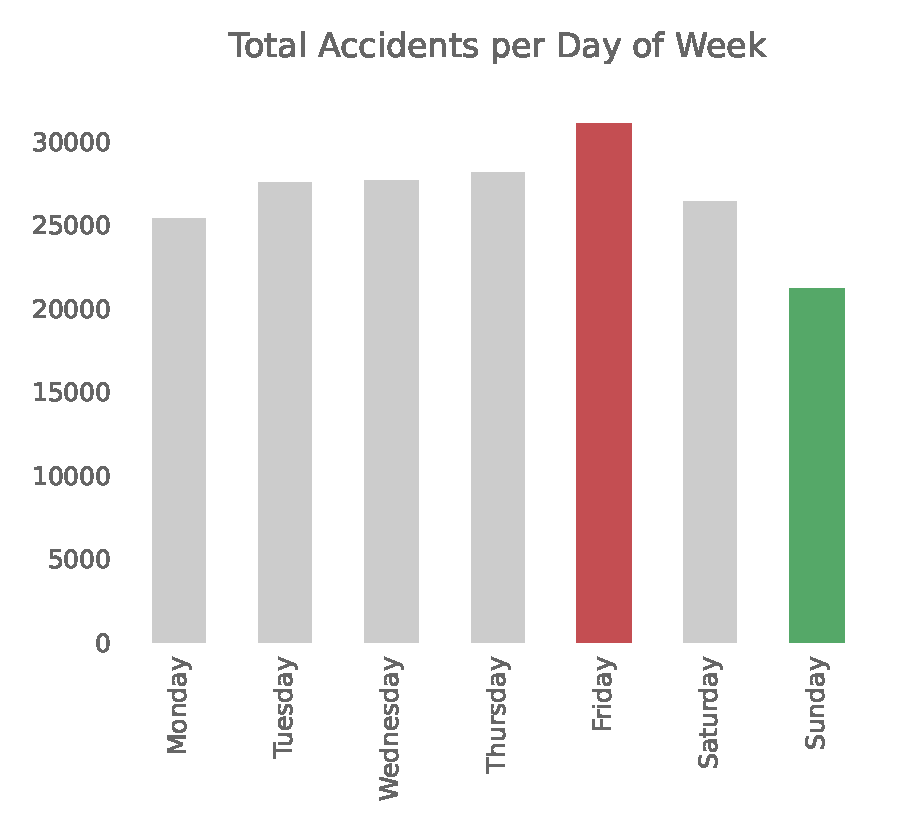
\includegraphics[height=0.7\textheight]{plot_day_of_week.eps}\label{fig:day_of_week}
    \end{figure}
}

\frame{
    \frametitle{Accidents happen more on peak hours}
    \begin{figure}
        \centering
        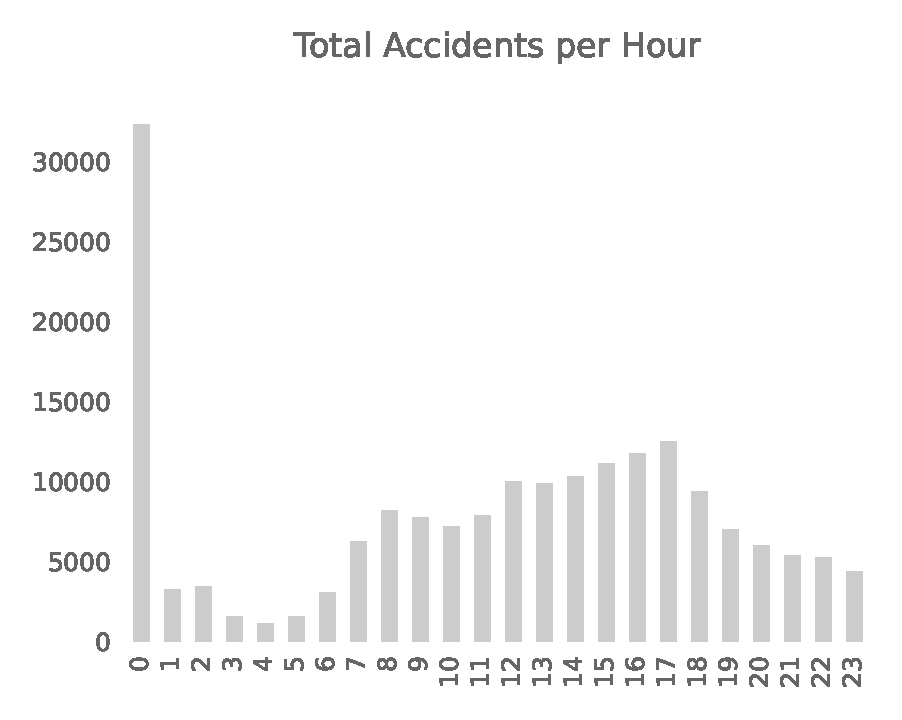
\includegraphics[height=0.7\textheight]{plot_hour.eps}
    \end{figure}
    The large amount of accidents at midnight (0 hour) should be missing values.
}

\frame{
    \frametitle{Accidents at intersections are more likely to be severe}
    \begin{figure}
        \centering
        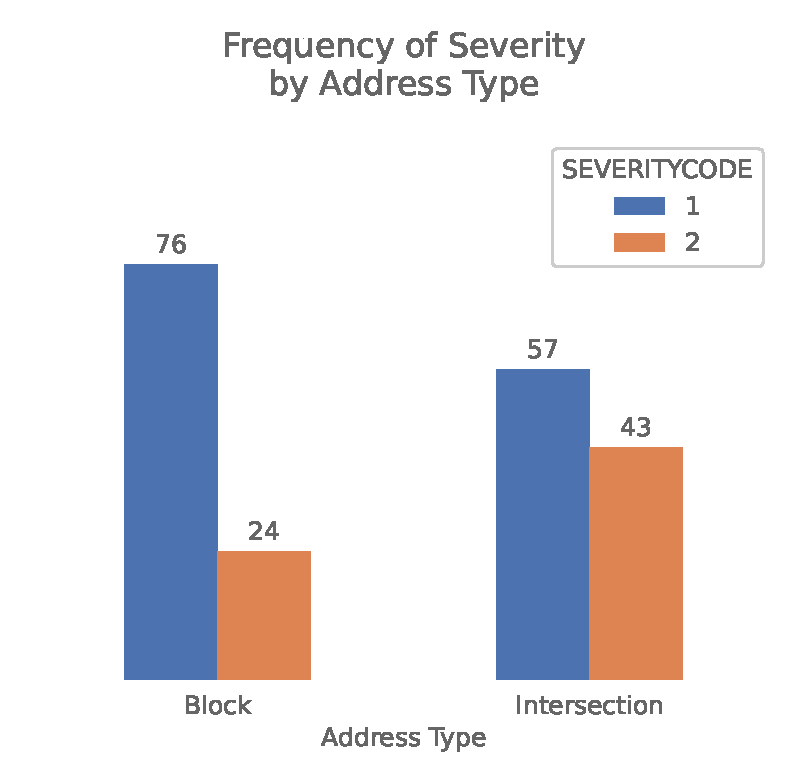
\includegraphics[height=0.7\textheight]{plot_addrtype.eps}\label{fig:addrtype}
    \end{figure}
}

\frame{
    \frametitle{Collision types influence severity}
    \begin{figure}
        \centering
        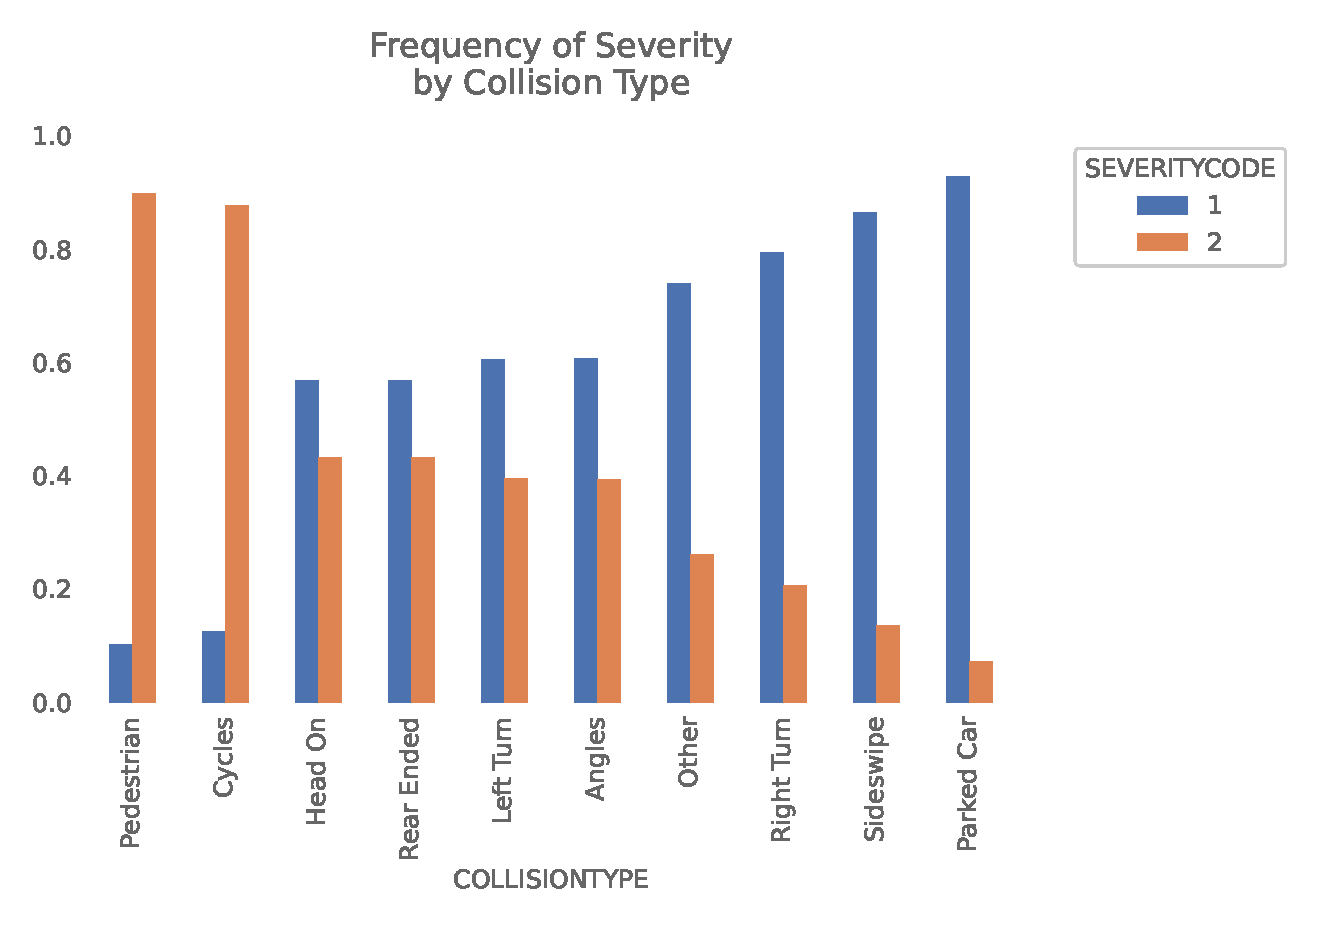
\includegraphics[height=0.7\textheight]{plot_collisiontype.eps}\label{fig:coltype}
    \end{figure}
    \begin{itemize}
        \item Collisions with pedestrians and bicycles are the most severe.
        \item Hitting a parked car almost always means no injury.
    \end{itemize}
}

\frame{
    \frametitle{Model performance}
    \begin{table}[h]
        \centering
        \begin{tabular}[c]{ c c c c c }
            \toprule
            Imbalanced Models & Precision & Recall & F1-score & AUC \\
            \midrule
            Logistic Regression & 0.75 & 0.75 & 0.71 & 0.79\\
            Random Forest & 0.73 & 0.75 & 0.72 & 0.77 \\
            XGBoost & 0.75 & 0.76 & 0.72 & 0.79 \\
            \midrule
            Balanced Models \\
            \midrule
            Logistic Regression & 0.75 & 0.67 & 0.68 & 0.79 \\
            Random Forest & 0.76 & 0.67 & 0.69 & 0.79 \\
            XGBoost & 0.76 & 0.67 & 0.68 & 0.79 \\
            \bottomrule
        \end{tabular}
        \caption{Weighted average precision, recall, f1-score and AUC for the models.\label{tab:metrics}}
    \end{table}
}

\frame{
    \frametitle{XGBoost performance}
    \begin{figure}
        \centering
        \begin{minipage}{.5\textwidth}
            \centering
            \includegraphics[width=0.9\linewidth]{plot_xgb_confmatrix}
        \end{minipage}%
        \begin{minipage}{.5\textwidth}
            \centering
            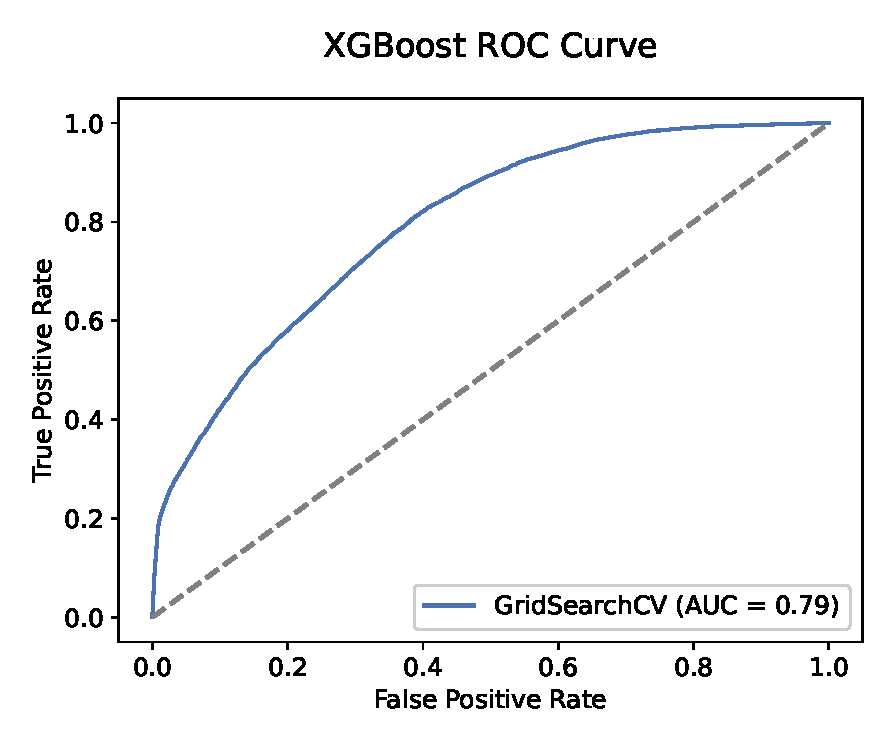
\includegraphics[width=0.9\linewidth]{plot_xgb_roc}
        \end{minipage}
    \end{figure}
}

\frame{
    \frametitle{XGBoost most important features}
    \begin{figure}
        \centering
        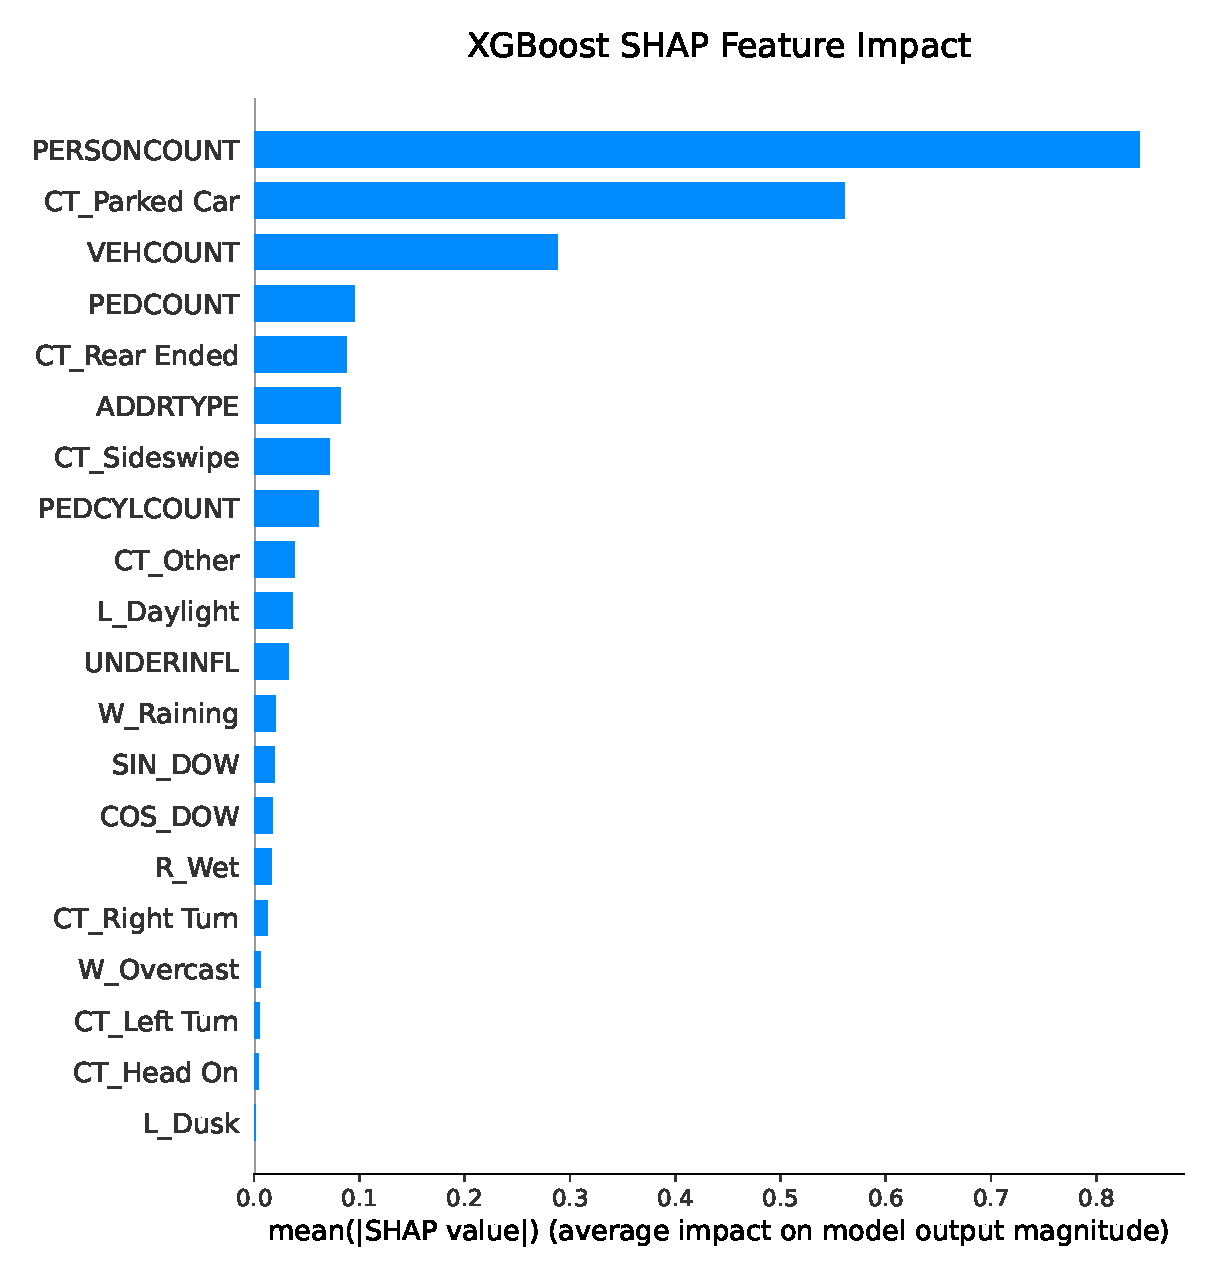
\includegraphics[height=0.8\textheight]{plot_shap_bar}
    \end{figure}
}

\frame{
    \frametitle{How feature values impact XGBoost model output}
    \begin{figure}
        \centering
        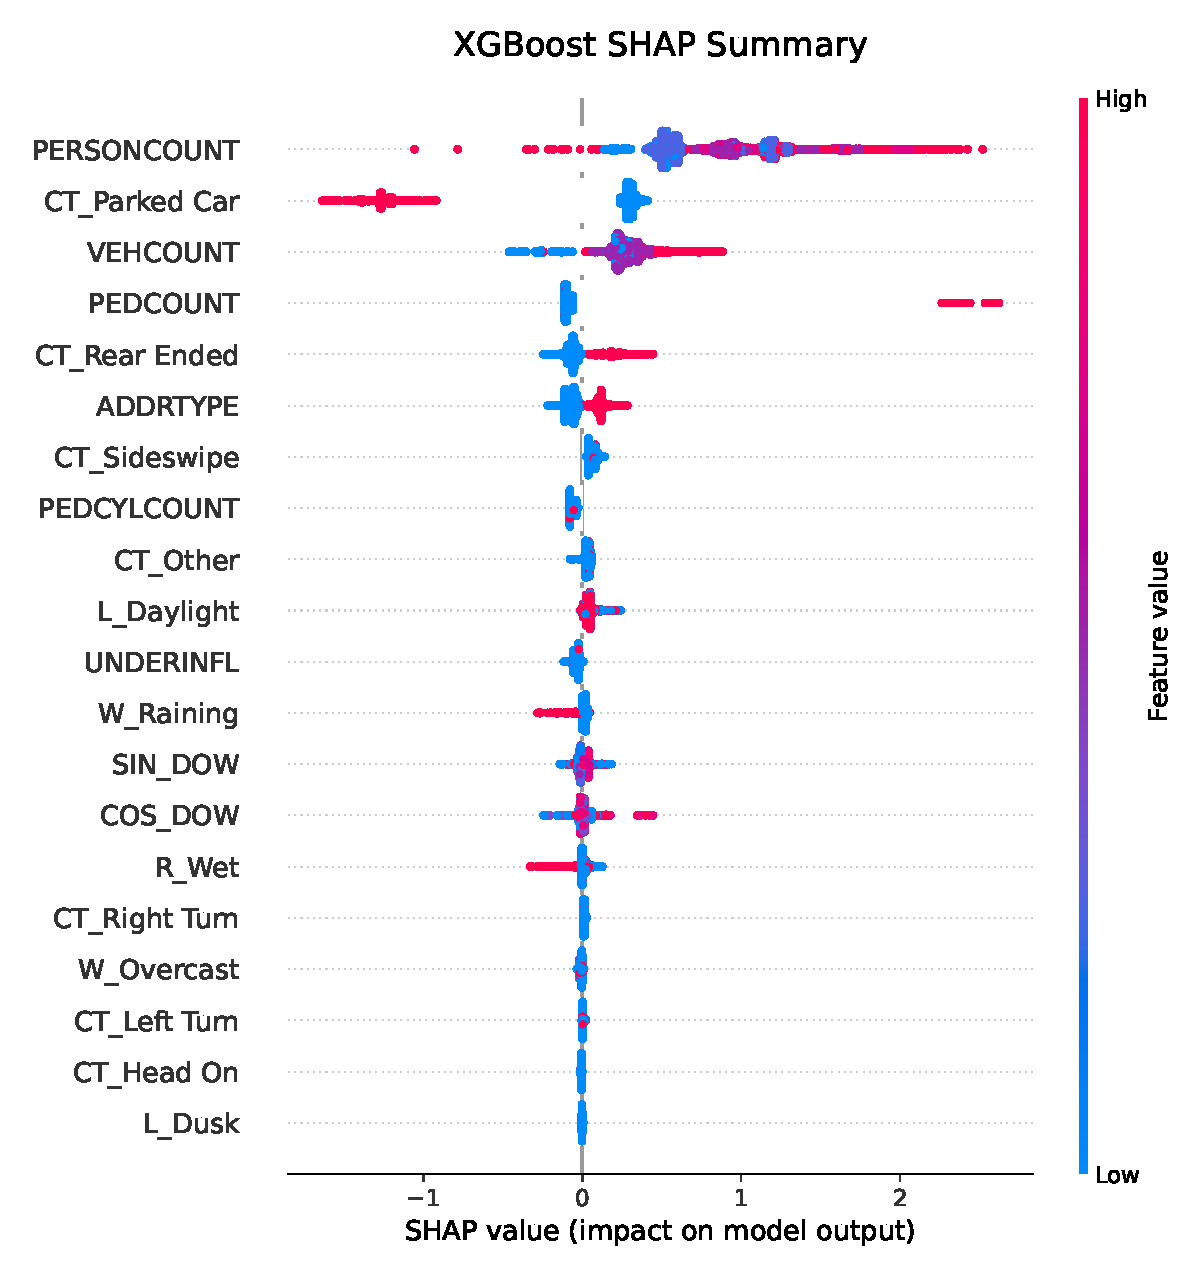
\includegraphics[height=0.8\textheight]{plot_shap_beeswarm}
    \end{figure}
}

\frame{
    \frametitle{Conclusion}
    \begin{itemize}
        \item We analyzed which factors influence accident severity.
        \item Machine learning models can predict severity based on open data.
        \item For future research:
            \begin{itemize}
                \item Use weather, traffic and data available in real time to predict the risk of accident.
            \end{itemize}
    \end{itemize}
}

\end{document}
